%% LaTeX2e class for student theses
%% sections/evaluation.tex
%% 
%% Karlsruhe Institute of Technology
%% Institute for Program Structures and Data Organization
%% Chair for Software Design and Quality (SDQ)
%%
%% Dr.-Ing. Erik Burger
%% burger@kit.edu
%%
%% Version 1.3.5, 2020-06-26

\chapter{Shapley additive explanations (shap)}
\label{chap:SHAP}

\begin{figure}[H]
    \centering
    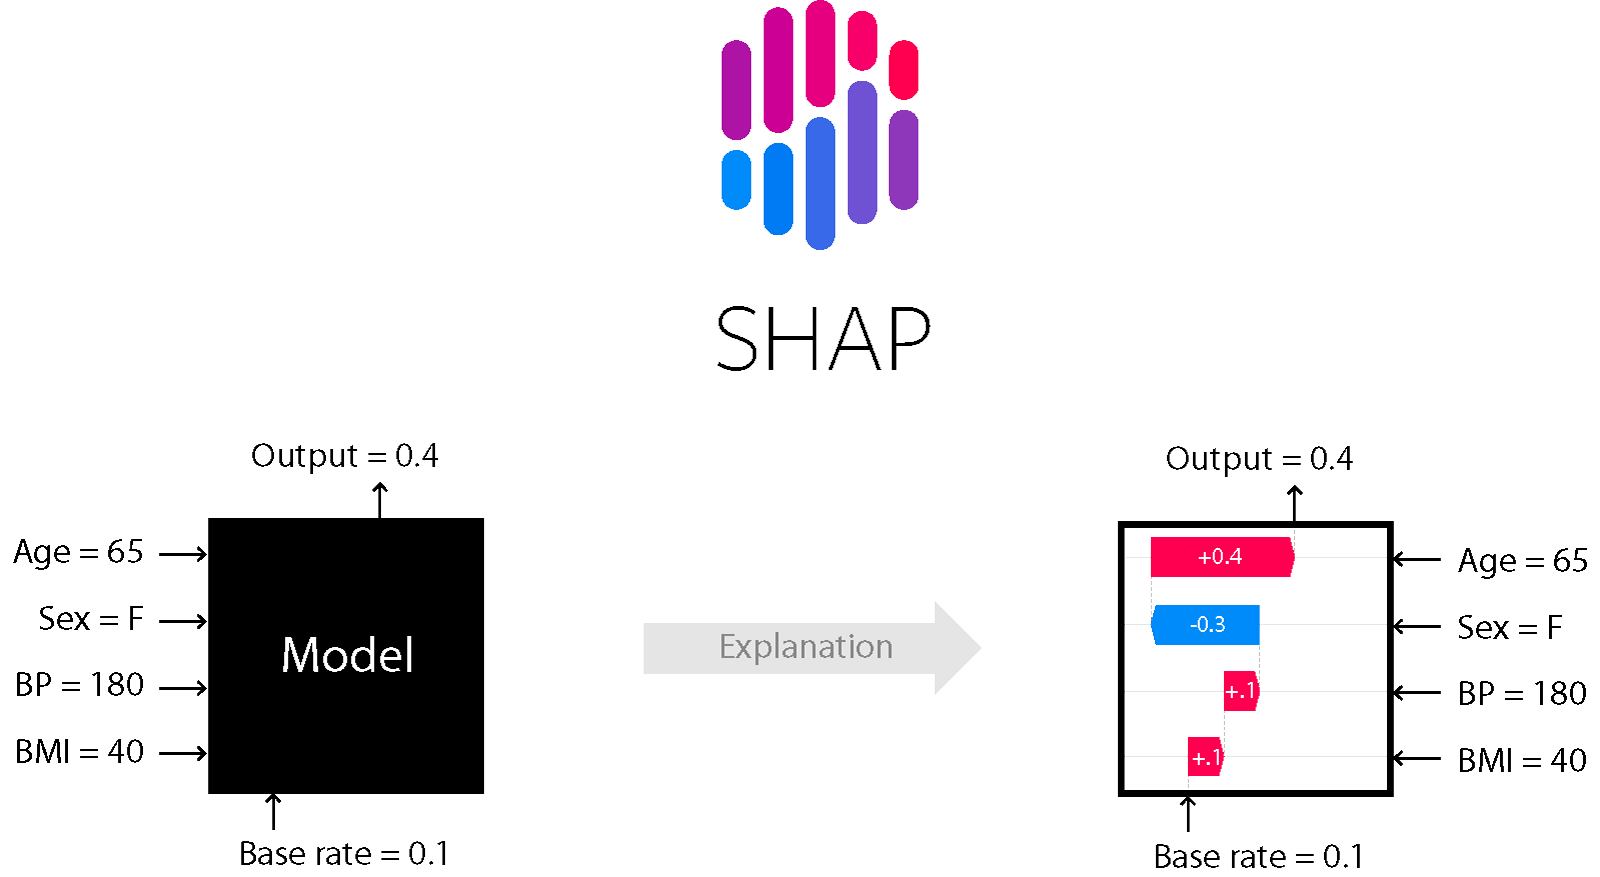
\includegraphics[width=\linewidth]{images/04_shap/ShapExplanationVisualized.png}
    \caption{Visualization of a shap explanation \cite{shapDocs}}
    \label{fig:shap_visualization}
\end{figure}


\section{General idea}

The human mind is astonishingly good at detecting patterns. It achieves this at an incredible rate still unmatched by our most powerful supercomputers \cite{patternRecognitionPsychology}. The issue is, that once a pattern is recognized, it gets rather hard to \enquote{forget} it even if it is a so called \enquote{false pattern}. This false pattern recognition is called apophenia and is considered a massive roadblock to creating an explanation model, because it severely limits the ability to understand the explanation model when presented to the user. If the user thinks he understood the explanation model and then gets another example explanation which contradicts his understanding of the explanation model, psychologically this is very confusing. 

\vspace{0.5cm}

A simple solution to this problem is to aid the human pattern recognition by defining rules that cannot be broken inside the approximation model. We will go over detail about these rules and why they make sense. This obviously doesn't eliminate the risk of apophenia but should decrease it significantly.

\vspace{1cm}

\textit{Please note that the psychological aspect was not explored in detail by the original shap paper. This is my own interpretation and argumentation as to why their work is a revolutionary approach to balance accuracy and interpretability in the context of neural network explanations. This is done because my work tries to improve the interpretability of the explanations by tackling above mentioned psychological barriers.}

\section{Competitive Game Theory}
\label{section:compGameTheory}

Game theory is a simple concept, where you study mathematical models of the interplay between rational decision makers. The most known example is the prisoners dilemma shown in \autoref{fig:prisonersDilemma}. 

\begin{figure}[H]
    \centering
    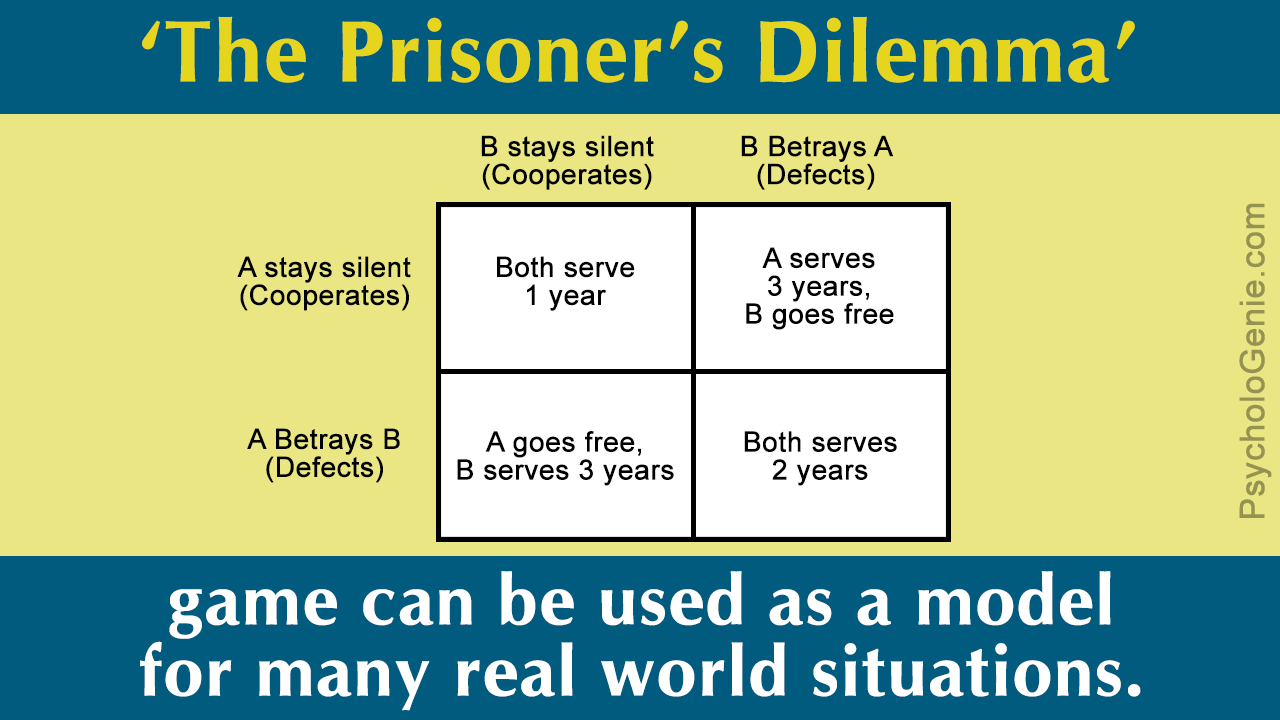
\includegraphics[width=\linewidth]{images/04_shap/Prisoners dilemma.png}
    \caption{Prisoners Dilemma \cite{psychologenie_2014}}
    \label{fig:prisonersDilemma}
\end{figure}

Game theory looks at how everyone should behave individually for the best outcome, and how a group of people should behave for the best outcome. The differences can then be discussed and often yield interesting properties. Competitive game theory is a subcategory of game theory, where a positive outcome for one \enquote{player} yields a negative outcome for another.

In our text classifications, this concept is used to determine the influence text-snippets have on the classification. Shap looks at the \textit{individual} influence of a single word, and then at how its context influences its meaning. For example the following text: "Jesus word is the word of God" will most likely be classified as being nearly 100\% christian, \textit{instead of being atheist}. If we remove the word Jesus from the text, it becomes as follows: "word is the word of God" which will also most likely be classified as nearly 100\% christian. Therefore individually, the word \textit{Jesus} does not influence the classification, but we intuitively know that it very much does or at least should. To find a more accurate value, to take the context into account, Shap removes multiple words in different orders and then combines the classification score differences using competitive game theory to find a more accurate value for that text-snippet.

\section{Shapley Properties}
\label{section:shapleyProp}

The values which determine the influence of each element introduced into the original model are called \textbf{shapley values}. They satisfy three very important properties meant to improve the interpretability of the results:

\begin{itemize}
    \item \textbf{Local Accuracy: } For the original input, the approximation model exactly matches the output of the original model.
    \item \textbf{Missingness: } This property is very misleading and should not be considered important. As described in the original shap paper \cite{shapPaper}: If the missing of a feature in  the original model does not change the result of the original model, then it should not have any impact in the approximation model either. This seems to contradict the use of competitive game theory and it does. I will directly quote the author of the shap paper Scott M. Lundberg when asked about this: \vspace{0.5cm}\newline
    \textit{\enquote{The missingness property is really just a minor book-keeping property to close a loop hole. It is required since local accuracy is specified as a linear model and x' [The input of the approximated model] could in theory have some zero entries (meaning the input is already missing [in the original input]). These zero entries mean that local accuracy would still hold no matter what phi values correspond to those entries, so to have a unique solution we need to constrain them to be 0 (which is what we want since they are missing already and so have no impact). In practice for SHAP we will never consider a feature to already be perfectly missing unless that feature's value is constant over the whole background dataset \cite{slundbergMissingness}.}} \newline
    \vspace{0.5cm} \newline
    To sum it up, it means that if a feature, meaning an indivisible input, is not present in the original input, it shouldn't play any role in the explanation.
    \vspace{0.5cm} \newline
    \item \textbf{Consistency:} if the importance of a feature increases because the original model has changed, then its importance should not decrease in the explanation model. This property makes the results much more interpretable, because consistency is an important part of interpretability.
\end{itemize}

\section{Examples for explanations of text based classifiers}

\begin{figure}[H]
    \centering
    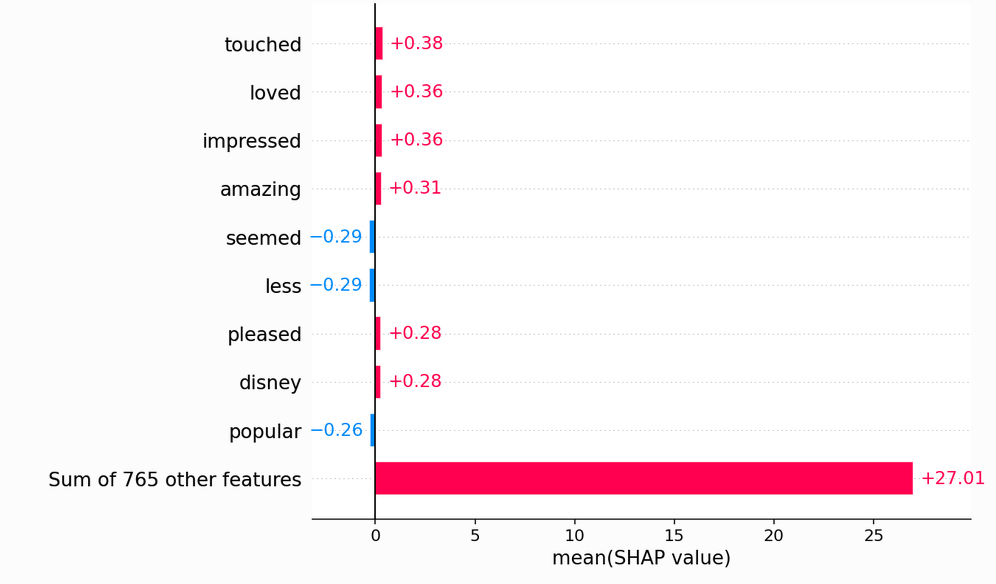
\includegraphics[width=\linewidth]{images/04_shap/ShapExplanationExample1.PNG}
    \caption{Shap explanation example \cite{shapDocs}}
    \label{fig:ShapExplEx1}
\end{figure}

In \autoref{fig:ShapExplEx1} we see the top 9 features which have the largest influence on the classification with their respective shapley values. These values are getting dwarfed by the sum of all other features, but it helps to give an idea about how the classifier works. If the top features should not be part of the classification process, we can suspect that something is wrong with the classification.


This can be rather difficult, especially, if words which only show their importance in their respective context are part of the top 10 most important features. This issue is one we are going to try to approach in \autoref{ch:Results} and suggest how to improve the interpretability of the explanation by using different text hierarchies.

% Example of where interpretability does not work

\subsection{Example where the explanation is difficult to understand because the context is missing.}
\label{section:ExplanationExample}

The following email has been classified as being 99\% christian:

\noindent\rule[0.5ex]{\linewidth}{1pt}
From: jenk@microsoft.com (Jen Kilmer)\\
    Subject: Re: Homosexuality issues in Christianity\\
    Organization: Microsoft Corporation\\
    Lines: 27\\
    
    In article <May.11.02.36.59.1993.28108@athos.rutgers.edu>\\ dps@nasa.kodak.com writes:\\
    >In article 15441@geneva.rutgers.edu, loisc@microsoft.com (Lois\\ Christiansen) writes:\\
    
    >|>he can, especially homosexuality.  Let's reach the homosexuals for\\ Christ.\\
    >|>Let's not try to change them, just need to bring them to Christ.  If He\\
    >|>doesn't want them to be gay, He can change that.  [....]\\
    
    >don't hate the people.  I don't.  I don't hate my kids when they do\\
    >wrong either.  But I tell them what is right, and if they lie or don't\\
    >admit they are wrong, or just don't make an effort to improve or\\
    >repent, they get punished.  I think this is quite appropriate.\\
    
    Note the difference here. One is saying, if *Christ* disagrees with\\
    a Christian being gay, *Christ* can change that.\\
    
    The other is saying, if *I* think being gay is wrong, that a Christian\\
    cannot be gay, *I* need to tell them to change.\\
    
    
    As Lois said, and as before her Paul wrote to the believers in Rome,\\
    WHO ARE YOU TO JUDGE ANOTHER'S SERVANT?\\
    
    -jen\\
    
    --
\cite{Newsgroups20}\\
\noindent\rule[0.5ex]{\linewidth}{1pt}

The classification is obviously correct, we will now run shap trying to find out why that classification score was reached:
\begin{table}[H]
    \centering
        \begin{tabular}{c|c}
                Feature name & Feature importance \\ \hline
                rutgers & 0.040224 \\
                athos & 0.036232 \\
                geneva & 0.030274 \\
                1993 & 0.025009 \\
                christ & 0.022898 \\
                article & 0.021479 \\
                writes & 0.019735 \\
                com & 0.019473 \\
                paul & 0.016807 \\
                don't & 0.014403 \\
                nntp-posting-host & 0.010084 \\
                nntp-posting-host & 0.010084 \\
                atheism & 0.008166 \\
                christian & 0.00862 \\
                christianity & 0.008166 \\
                christians & 0.00797
            \end{tabular}
            \caption{Example where it is difficult to interpret what the classifier does.}
            \label{tab:example_bad_interpretation}
\end{table}

Here we find out, that the classification is being done by looking at the header, the email provider. If studied in more detail, it would become clear, that the training dataset is flawed, all christian emails come from the same email provider. The classifier is not doing what it should, it reaches the correct classification, but if the header is missing, the classification result would become mostly random. Coming to this conclusion takes a lot of work though, because if we didn't provide the original text, you would be confused about the presence of words like \enquote{rutgers}, \enquote{athos} or \enquote{don't}. These are so dependent on their context, that by themselves they do not provide any information at all. This problem is particularly apparent for text-classifiers and are the reason we chose them. In \autoref{ch:Results} we will suggest a method to remedy that particular issue.

\vspace{1cm}

We will now present the framework which was developed to  help analyse multiple explainers.